\documentstyle[psfig]{article}

%\psdraft

\begin{document}

\title{Theory behind {\sf paircomp}}
\author{C. Titus Brown\\Caltech}
\date{April 2004}
\maketitle

\tableofcontents

\section{Introduction}

This is a miscellaneous collection of the math ``theory'' behind
{\sf paircomp}/{\sf seqcomp}-style fixed-width-window matching.
The first section, on Monte Carlo sequence matching probabilities,
was mostly written back in 2000, at the request of my advisor, Eric
Davidson; the second section, on building a score for matches, was
written in late 2003, at the request of Erich Schwarz.

Tristan De Buysscher is the author of the {\sf seqcomp} program that
I used during this period, and my co-conspirator in this matter.

\section{Monte Carlo sequence matching probabilities}

The problem of finding a match of exactly M base pairs of a particular W-mer
reference sequence in some subsequence of L equiprobably chosen bases is
equivalent to the following problem: pick W balls from a large collection of
red and blue balls, with probability $p = { 1 \over 4 }$ of picking a blue ball
and probability $q = {3 \over 4}$ of picking a red ball, and repeat $(L - W +
1)$ times, looking for exactly $M$ blue balls of the $W$ total chosen.

The probability of finding exactly $M$ blue balls out of the $W$ chosen
is a simple binomial calculation:
\[
P(M, W) = { W \choose M } p^{M} q^{W - M}
\]
The corresponding distribution peaks at the mean, $Wp$, and has variance
$Wpq$.  (figure)

When repeating $L$ times ($L >> W ==> L-W+1 \approx L$) we can ask for
the probability of getting one or more candidate matches by calculating
the Poisson probability of exactly 0 matches and then subtracting it from
1:
\[
{\cal P}_L(E) = 1 - \exp(-\lambda(L))
\]
where $E$ is the occurrence of one or more matches, and the formula is for
the Poisson distribution at $x=0$.  The Poisson parameter $\lambda$ is
a function of the size of the sequence $L$ (equivalently,
the number of candidate matches generated), and can be chosen by setting
$\lambda$ equal to the mean number of events.  For a binomial
distribution bin(n, p) the mean is $np$, and if
we require that this match the mean of the Poisson distribution, we find
that
\[
\lambda(L) = Lp
\]
and then
\[
{\cal P}_L(E) = 1 - \exp(-L p)
\]

By way of intuitive confirmation, note that the distribution (figure)
asymptotically approaches 1, so that the probability of generating at
least one match converges to one as the number of tries approaches infinity;
as well, the probability of getting a match in few tries (given a rare
event, equivalently a small $p$) is approximately 0.

\begin{figure}
\psfig{file=R/trials.ps,width=5in,angle=-90}
\caption{Probability of seeing one or more motif matches for a given
sequence length across matches of 15/20 to 20/20.}
\end{figure}

\subsection{Distribution of maximum matches}

Now suppose we have an ensemble of sequences of length L and we would
like to describe the distribution of {\em maximum} matches to a W-mer
on members of the ensemble.
That is, given a particular W-mer matched against every W-length
subsequence of each sequence in the ensemble, what is the distribution
of best matches to the W-mer across the ensemble?

To describe this in terms of the probability distribution derived above,
we need only consider two types of events: the event $E$ in which at least
one subsequence has M matches, and the event $NE$ in which no subsequences
have (M + 1) or more matches.  Then the probability that the best match
to a subsequence of an L-length sequence is $M$ is
\[
W_L(E) (1 - W_L(NE))
\]
Now, $W_L(E) = {\cal P}_L(E)$, and $W_L(NE) = {\cal P}_L(NE)$ which
can be generated by replacing the probability $p$ of generating $M$ matches
with the probability $p_WM = \sum^W_{i=M+1} bin(W, i)$, that is,
the probability that no more than M matches are generated in a given
attempt.

\begin{figure}
\psfig{file=R/bestmatches-20.ps,width=5in,angle=-90}
\psfig{file=R/bestmatches-50.ps,width=5in,angle=-90}
\caption{Distribution of best matches for windows of size 20 and 50,
for sequences of length $10^6$.}
\end{figure}

The resulting probability distribution is graphed for a fixed $L = 1e6$,
below.

\begin{figure}
\psfig{file=R/window=20.ps,width=5in,angle=-90}
\psfig{file=R/window=50.ps,width=5in,angle=-90}
\caption{Expected best matches, according to sequence length,
for two different match-window sizes: top = 20, bottom = 50.}
\end{figure}

\subsection{Distribution of best matches in diverging sequences}

Suppose that you have a sequence of L bases, each of which is
mutated with a probability $p$ (which can be related to a Poisson
rate of mutation and a waiting time via an exponential, as above).
The problem now changes so that you start with a full set of matches
and then randomly alter the selection of matches with some probability.
Accounting for backmutations, then, the probability that any given
base still matches is
\[
P(p) = (1 - p) + \frac{p}{4} = 1 - \frac{3p}{4}
\]
-- the probability of no mutation plus the probability of back mutation.
Checking boundary conditions reveals the expected results: for $p=0$
(no mutation), $P = 1$; for $p=1$ (no unchanged bases), $P=\frac{1}{4}$,
random (as discussed above).

\begin{figure}
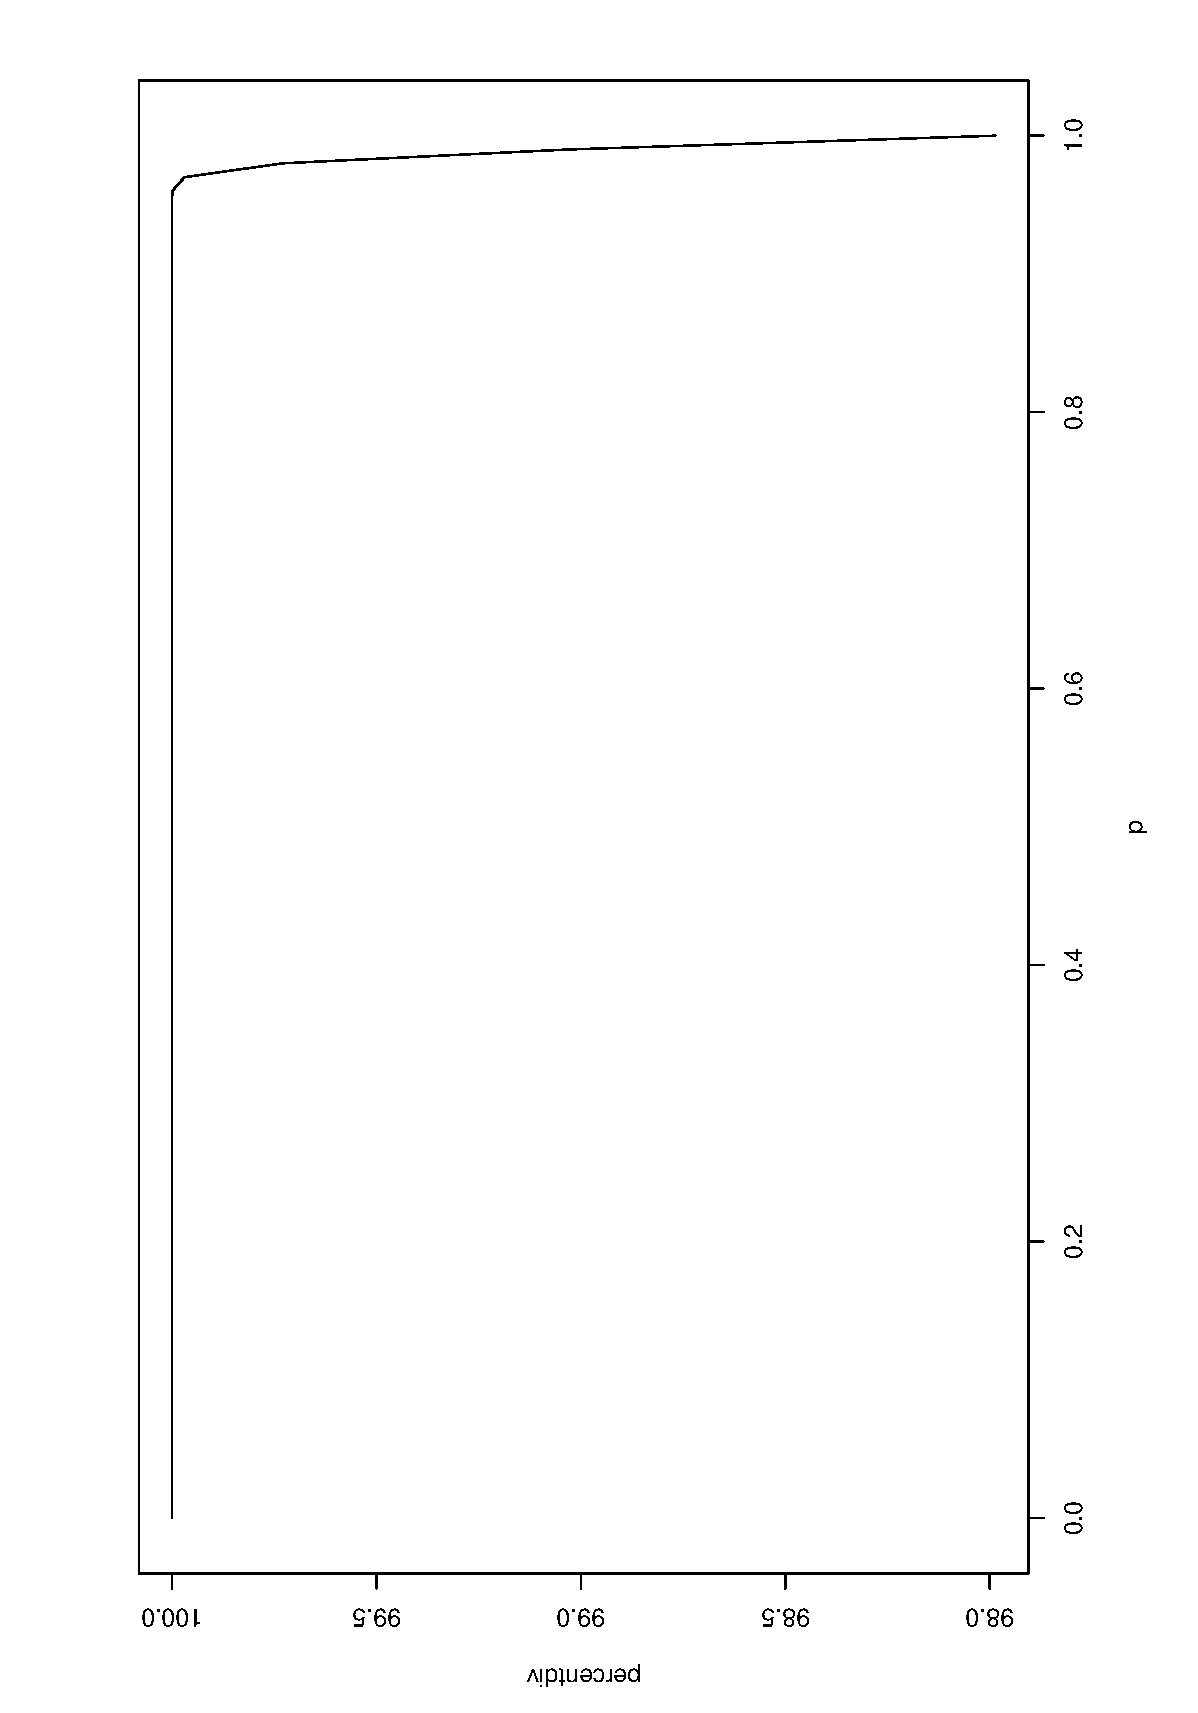
\psfig{file=R/divergedist-20.ps,width=5in,angle=-90}
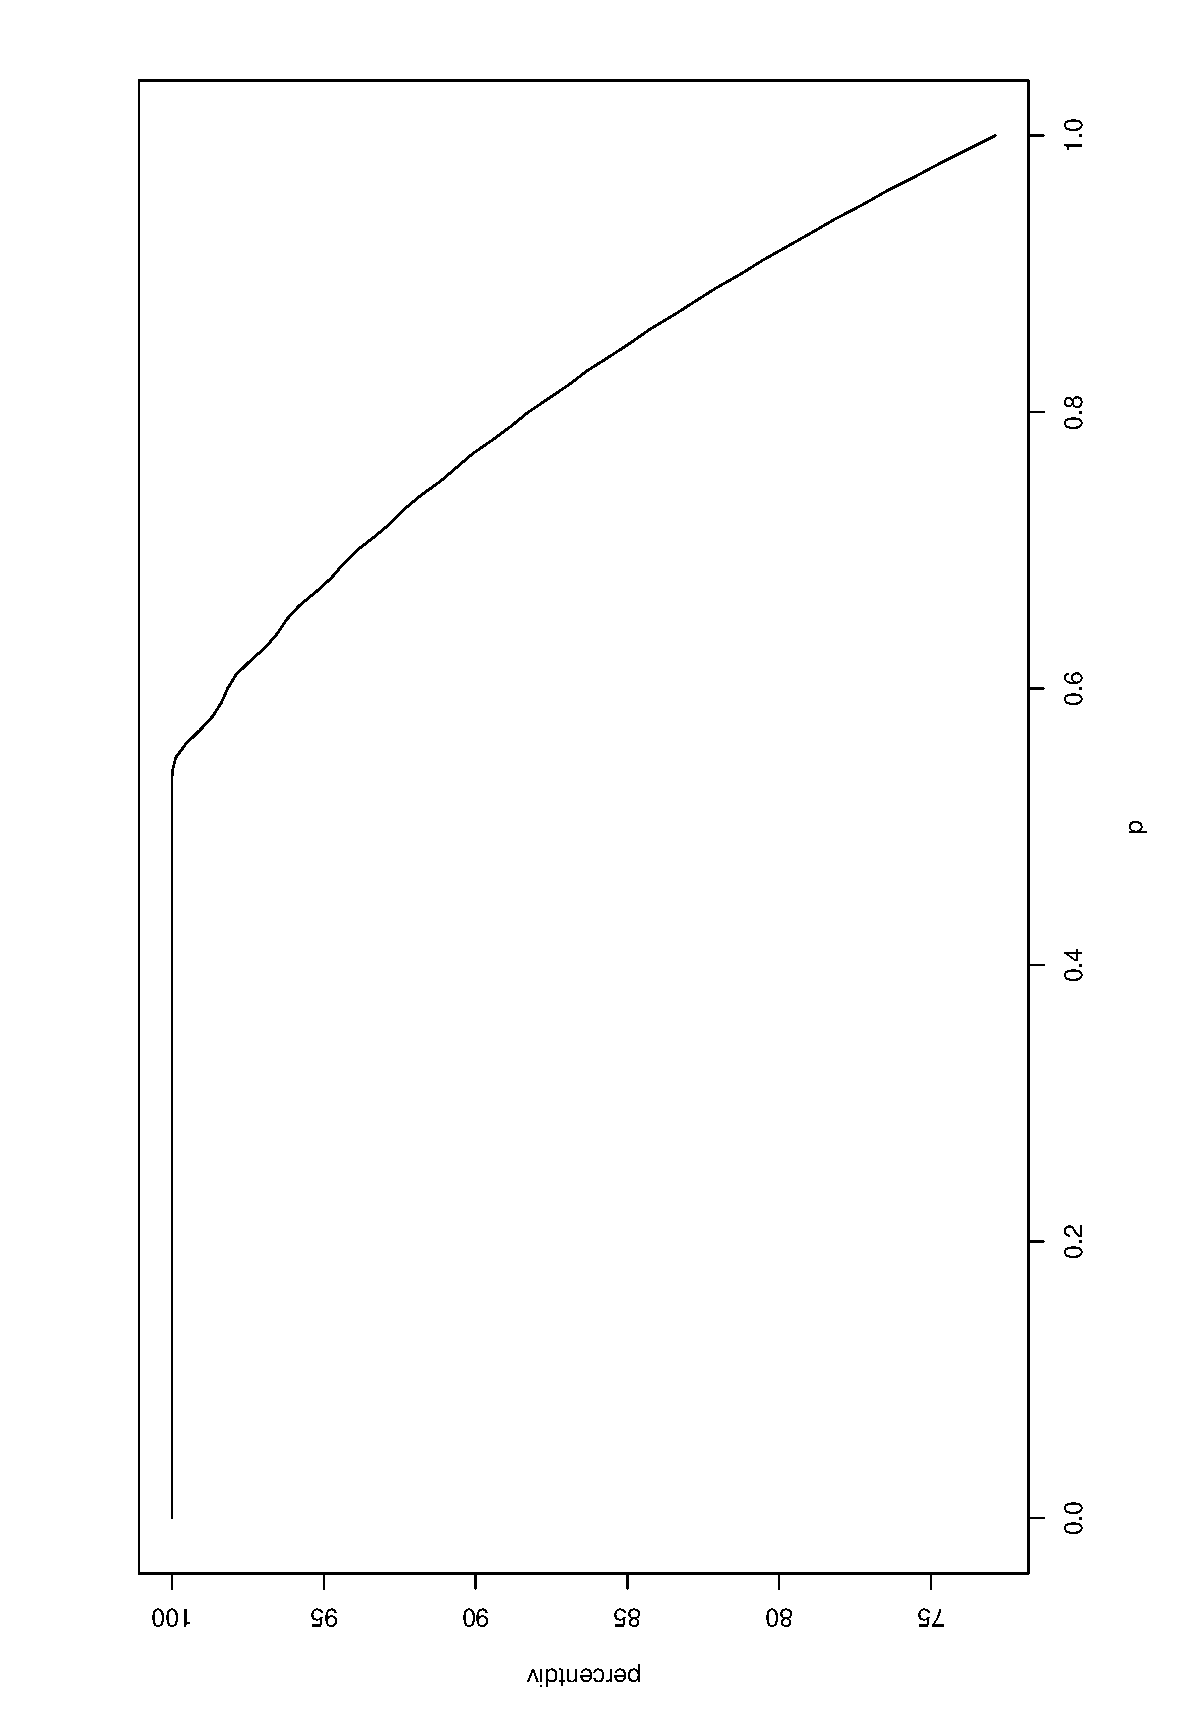
\psfig{file=R/divergedist-50.ps,width=5in,angle=-90}
\caption{Expected best matches for a sequence of length $10^{12}$,
with windowsize 20 (top) and 50 (bottom),
for different divergences.  Divergences are
measured here as values of $p$, the probability that any given
base pair is mutated.}
\end{figure}

\section{Scoring matches}
Assume a match between two sequences $a$, $b$ of length $N$.
The probability of these two sequences being generated randomly
(hypothesis $R$) is
\[
p(a, b | R) = \prod_i q_{a_i} \prod_j q_{b_j}
\]
where $q_{a_i}$ is the probability of the i'th nucleotide in sequence $a$;
for a equiprobable distribution of bases,
\[
q_{a_i} = q_{b_j} = p_A = p_C = p_G = p_T = {1 \over 4}
\]
The probability of these two sequences being aligned (hypothesis
M) assuming independence between bases is that
\[
p(a, b | M) = \prod_i p_{a_i,b_i}
\]
which must be chosen according to some model of nucleotide matching.  For
comparative sequence analysis of noncoding regions, this probability
corresponds to our belief that an identity between two nucleotides
indicates conservation for functional reasons as opposed to accidental
failure to diverge.  Since we have no reason
to bias ourselves for or against any particular nucleotide identity, we can
pick a single parameter $\lambda$ to represent the likelihood for
all four bases that the nucleotide match is due to conservation,
which gives us
\begin{eqnarray*}
p_{a_i,b_i} &=& \delta_{a_i,b_i} \left({1 \over 16} + {3 \lambda \over 16}\right) + 
            (1 - \delta_{a_i,b_i}) \left({1 \over 16} - {\lambda \over 16}\right) \\
&=& \delta_{a_i,b_i} \left({ 1 + 3\lambda \over 16}\right) +
            (1 - \delta_{a_i,b_i}) \left({ 1-\lambda \over 16}\right) \\
\end{eqnarray*}
where $\delta_{a_i,b_i}$ is the identity matrix, 1 when $a_i=b_i$ and
 0 otherwise, and
$\lambda \in [0,1)$.  This can be broken down into two probabilities,
$p_{\rm match}$ and $p_{\rm mismatch}$:
\[
p_{\rm match} = { 1 + 3\lambda \over 16 },
p_{\rm mismatch} = { 1 - \lambda \over 16}
\]
Note that for $\lambda=0$ -- no identity due to conservation -- these joint
probabilities equal the independent probabilities, and for $\lambda=1$
the probability of any given non-identitical match is 0, which will certainly
be counter to observation for any inhomogeneous sequence regions.

Given these two probability measures, we can now construct a log-ratio
score according to Durbin et al., p13-14:
\begin{eqnarray*}
s(a,b) &=& \log { p(a,b | M) \over p(a,b | R)} \\
&=& \log \left(\prod_i { p_{a_i,b_i} \over q_{a_i} q_{b_i} }\right) \\
&=& \sum_i \log {p_{a_i,b_i} \over q_{a_i} q_{b_i} } \\
&=& \sum_i \log p_{a_i,b_i} - \log q_{a_i} q_{b_i}  \\
\end{eqnarray*}
This can easily be calculated for any particular value of $\lambda$;
for $M$ nucleotide matches of an $N$-length sequence,
\[
s(a,b) = M \log p_{\rm match} + (N - M) \log p_{\rm mismatch} -
\sum_{i} \log q_{a_i} q_{b_i}
\]
In the simplest case, for a uniform distribution of nucleotides in the
background sequence, $q_{a_i} = q_{b_i} = {1 \over 4}$,
\[
\sum_i \log q_{a_i} q_{b_i} = \sum_i 2 \log {1 \over 4} = -4 N
\]
and so
\[
s(a,b) = M \log p_{\rm match} + (N - M) \log p_{\rm mismatch} + 4N
\]
This score has been implemented in the associated {\tt seqcomp-score.py} file.

\subsection{Discussion}

The score developed above relies on a few assumptions:
\begin{itemize}
\item individual nucleotide matches can be considered independently of
their surroundings;
\item A, C, T, and G are equally likely to be conserved.
\end{itemize}

The parameter $\lambda$ can be thought of as a kind of inverse distance
measure: the closer it is to 0, the more randomized the sequences from
which the matches were taken, and the closer it is to 1, the stronger
the contribution from conservation.  However, this parameter is essentially
irrelevant: as long as it is held constant when comparing scores for
different matches, the scores will be comparable, even for different
background sequence distributions.

This score is easily extended for multiple sequence analysis, e.g.
three-way comparison of matches.  However, for each additional sequence, a
new $\lambda$-like parameter is needed; it is unclear exactly what this
means, however, in the context of actual scoring!

Finally, note that other than being readily calculable, the one major
advantage this score has over the previously developed statistics for
comparative sequence analysis is that it can easily take into account
different background nucleotide probabilities, thus alleviating problems
caused by e.g. AT-rich sequences in {\em C. elegans}.

\end{document}